% UTF-8 encoding
% Compile with latex+dvipdfmx, pdflatex, xelatex or lualatex

\documentclass[hyperref, UTF8]{ctexart}
\usepackage{amssymb}
\usepackage{amsmath}
\usepackage{graphicx}
\usepackage{subfigure}
\usepackage{geometry}
\usepackage{caption}
\usepackage{upgreek}
\newcommand{\volt}{{\rm V}}
\newcommand{\source}{{\rm S}}
\newcommand{\second}{{\rm s}}
\newcommand{\ampere}{{\rm A}}
\newcommand{\milliampere}{{\rm mA}}
\newcommand{\hertz}{{\rm Hz}}
\newcommand{\ohm}{\Omega}
\newcommand{\kiloohm}{{\rm k}\Omega}
\newcommand{\watt}{{\rm W}}
\newcommand{\kilowatt}{{\rm kW}}
\newcommand{\degree}{^{\circ}}
\newcommand{\farad}{{\rm F}}
\newcommand{\microfarad}{{\rm \upmu F}}
\newcommand{\millifarad}{{\rm mF}}
\newcommand{\henry}{{\rm H}}
\newcommand{\J}{{\rm j}}
\newcommand{\D}{{\rm d}}
\newcommand{\E}{{\rm e}}

\title{电子学基础——第七次作业}
\author{LXQ}
\date{2019.11.11}

\geometry{left=2.0cm, right=2.0cm, top=2.5cm, bottom=2.5cm}
\linespread{1}

\begin{document}

\maketitle

\paragraph{3.1}
Plot the I/V characteristic of the circuit shown in Fig. 3.63.

\begin{figure}[!htb]
    \centering
    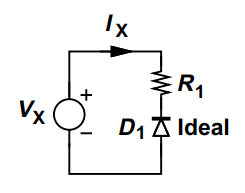
\includegraphics[width=0.163\textwidth]{f3-63.png}
    \caption*{Figure 3.63}
\end{figure}    

\paragraph{Solution} The figure is shown in Figure p3.1.

\begin{figure}[!htb]
    \centering
    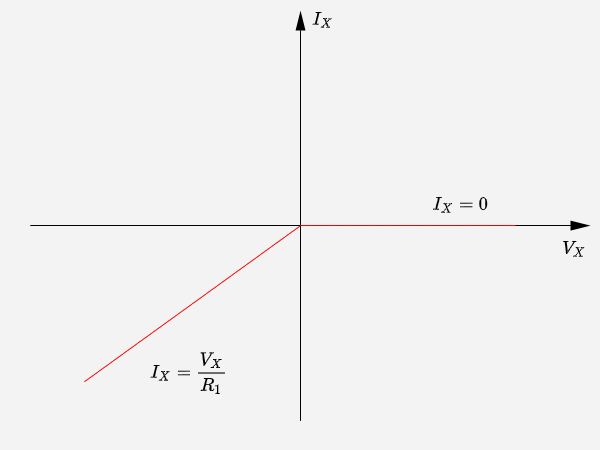
\includegraphics[width=0.400\textwidth]{p3-1.png}
    \caption*{Figure p3.1}
\end{figure}    

\paragraph{3.2}
If the input in Fig. 3.63 is expressed as $V_X = V_0\cos \omega t$, plot the current flowing 
through the circuit as a function of time.

\paragraph{Solution}
$$
I_X = \left\{ \begin{aligned} 
    & \frac{V_0}{R_X} \cos \omega t, & \frac{4k\pi + \pi}{2\omega} \le t < \frac{4k\pi + 3\pi}{2\omega} \\
    &  0, & \frac{4k\pi + 3\pi}{2\omega} \le t < \frac{4k\pi + 5\pi}{2\omega} 
\end{aligned}
\right.
$$
The figure is shown in Figure p3.2.

\begin{figure}[!htb]
    \centering
    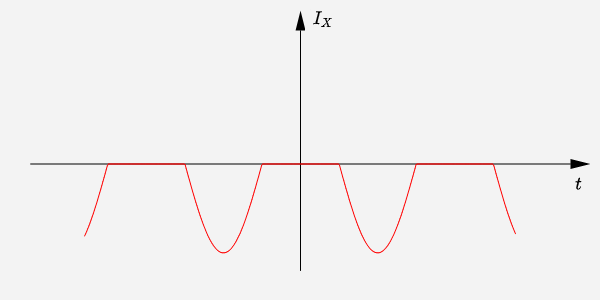
\includegraphics[width=0.400\textwidth]{p3-2.png}
    \caption*{Figure p3.2}
\end{figure}

\paragraph{3.20}
In the circuits depicted in Fig. 3.72, assume $I_{in}=I_0 \cos \omega t$, where $I_0$ is
relatively large. Plot $V_{out}$ as a function of time using a constant voltage diode model.

\paragraph{Solution} The figures as shown in Figure p3.20

(a)
$$
V_{out} = \left\{ \begin{aligned}
    & I_{in}R_1, & -I_{in}R_1+V_B < V_{D,on} \\
    & V_B - V_{D,on}, & -I_{in}R_1+V_B \ge V_{D,on} 
\end{aligned} \right.
$$

(b)
$$
V_{out} = \left\{ \begin{aligned}
    & I_{in}R_1 + V_B, & I_{in}R_1+V_B > -V_{D,on} \\
    & - V_{D,on}, & I_{in}R_1+V_B \le V_{D,on} 
\end{aligned} \right.
$$

(c)
$$
V_{out} = \left\{ \begin{aligned}
    & V_B + I_{in}R_1, & -I_{in}R_1 < V_{D,on} \\
    & V_B - V_{D,on}, & -I_{in}R_1 \ge V_{D,on} 
\end{aligned} \right.
$$

\begin{figure}[!htb]
    \centering
    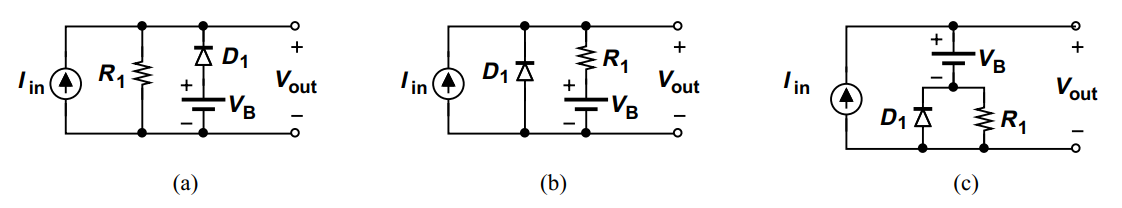
\includegraphics[width=0.748\textwidth]{f3-72.png}
    \caption*{Figure 3.72}
\end{figure}    

\begin{figure}[!htb]
    \centering
    \begin{minipage}[t]{0.400\textwidth}
    \centering
    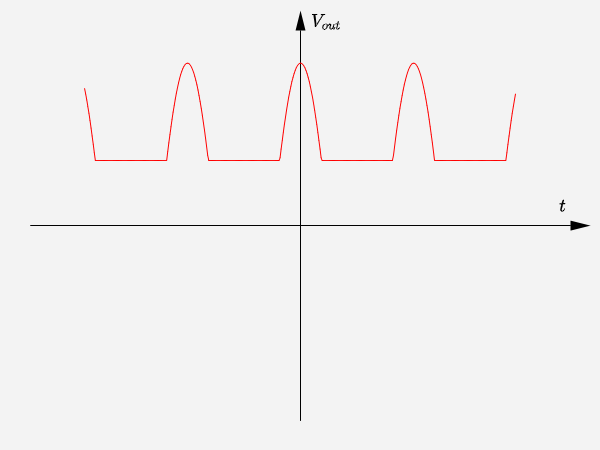
\includegraphics[width=1\textwidth]{p3-20-a.png}
    \caption*{(a)}
    \end{minipage}
    \\
    \begin{minipage}[t]{0.400\textwidth}
    \centering
    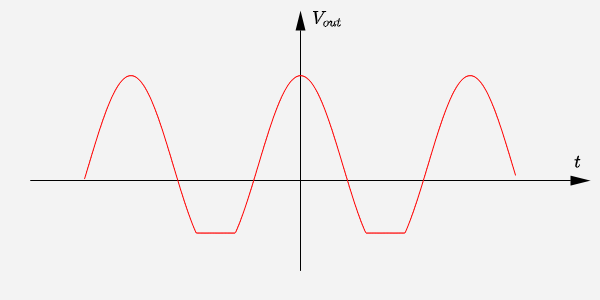
\includegraphics[width=1\textwidth]{p3-20-b.png}
    \caption*{(b)}
    \end{minipage}
    \begin{minipage}[t]{0.400\textwidth}
    \centering
    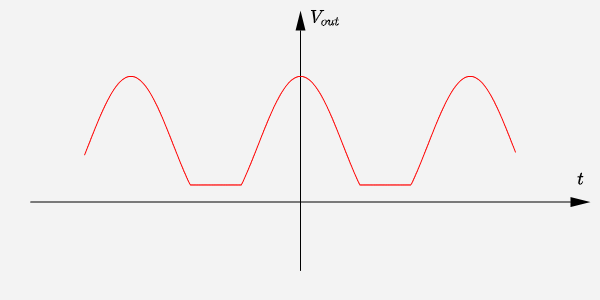
\includegraphics[width=1\textwidth]{p3-20-c.png}
    \caption*{(c)}
    \end{minipage}
    \caption*{Figure p3.20}
\end{figure}

\paragraph{6.12}
It is possible to define an "intrinsic time constant" for a MOSFET operating as a resistor: 
$$\tau = R_{on}C_{GS}$$
where $C_{GS} = WLC_{ox}$. Obtain an expression for $\tau$ and explain what the circuits 
designer must do to minimize the time constant.

\paragraph{Solution}
It is known that when a MOSFET works as a resistor, 
$$
I_D = \frac{1}{2} \mu _n C_{ox} \frac{W}{L} [2(V_{GS} - V_{th}) V_{DS} - V_{DS}^2] 
\approx \mu _n C_{ox} \frac{W}{L} (V_{GS} - V_{th}) V_{DS}
$$
$$
\therefore R_{on} = \mu _n C_{ox} \frac{W}{L} (V_{GS} - V_{th}) 
$$
$$
\tau = \mu_n C_{ox}^2 W^2 (V_{GS} - V_{th})
$$
Therefore, in order to minimize the time constant $\tau$, the designer should reduce the width $W$ 
and the capacitance $C_{ox}$.

\paragraph{6.13}
In the circuit of Fig. 6.37, $M_1$ serves as an electronic switch. If $V_{in} \approx 0$, 
determine $W/L$ such that the circuit attenuates the signal by only 5\%. Assume $V_G=1.8\volt$ and
$R_L = 100 \ohm$.

\begin{figure}[!htb]
    \centering
    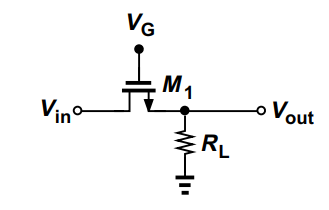
\includegraphics[width=0.219\textwidth]{f6-37.png}
    \caption*{Figure 6.37}
\end{figure}    

\paragraph{Solution}
    $$V_{out} = 0.95 V_{in} $$
    $$\therefore V_{DS} = 0.05 V_{in}, V_{GS} = 1.8 - 0.95 V_{in}$$
    $V_{in} \approx 0$, which means that the MOSFET works as a resistance:
    $$I_D = \frac{1}{2} \mu _n C_{ox} \frac{W}{L} [2(V_{GS} - V_{th}) V_{DS} - V_{DS}^2] 
\approx \mu _n C_{ox} \frac{W}{L} (V_{GS} - V_{th}) V_{DS} $$
    Assume $V_{th} = 0.5 \volt, \mu_n C_{ox} = 100 \milliampere / \volt^2$, and we can obtain that 
    $$  W/L = 1460 $$

\paragraph{6.25}
Calculate the bias current of $ M_1$ in Fig. 6.43 if $\lambda = 0$.

\begin{figure}[!htb]
    \centering
    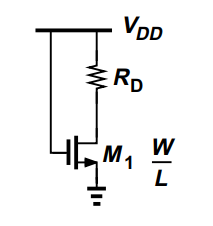
\includegraphics[width=0.142\textwidth]{f6-43.png}
    \caption*{Figure 6.43}
\end{figure}   

\paragraph{Solution}
$$I_D = \frac{1}{2} \mu_n C_{ox} \frac{W}{L}(V_{GS}-V_{th})^2$$
$$I_DR_D + V_{GS} = V_{DD}$$
$$\therefore I_D = \frac{1}{2} \mu_n C_{ox} \frac{W}{L}(V_{DD}-I_DR_D-V_{th})^2$$
The solution of the equation is: 
$$I_D =\frac{2R_DkV_S + 1 - \sqrt{4R_DkV_S-1}}{2kR_D^2}$$
where $k = \frac{1}{2}\mu_nC_{ox}\frac{W}{L}, V_S = V_{DD} - V_{th}$.

\paragraph{6.26}
Compute the value of $W/L$ for $M_1$ in Fig. 6.44 for a bias current of $I_1$. Assume $\lambda = 0$

\begin{figure}[!htb]
    \centering
    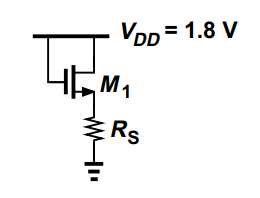
\includegraphics[width=0.173\textwidth]{f6-44.png}
    \caption*{Figure 6.44}
\end{figure}

\paragraph{Solution}
\begin{gather*}
\left\{ \begin{aligned}
    I_1 & =  \frac{1}{2} \mu_n C_{ox} \frac{W}{L}(V_{GS}-V_{th})^2 \\
    I_DR_S + V_{GS} & = V_{DD} \\
    V_S &= I_1R_S \\
    V_{GS} &= V_{DD} - V_S
\end{aligned} \right.
\end{gather*}
$$
\therefore \frac{W}{L} = \frac{2I_1}{\mu_n C_{ox} (V_{DD} - I_1R_S - V_{th})^2}
$$

\paragraph{6.27}
In Fig. 6.45, derive a relationship among the circuit parameters that guarantees $M_1$ operates at 
the edge of saturation. Assume $\lambda = 0$.

\begin{figure}[!htb]
    \centering
    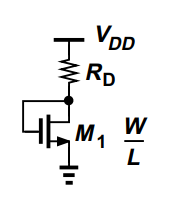
\includegraphics[width=0.115\textwidth]{f6-45.png}
    \caption*{Figure 6.45}
\end{figure}

\paragraph{Solution}
\begin{gather*}
    \left\{ \begin{gathered}
        I_D =  \frac{1}{2} \mu_n C_{ox} \frac{W}{L}(V_{GS}-V_{th})^2 \\
        V_{DD} = V_{GS} > V_{th} \\
        V_{GD} = I_DR_D < V_{th}
    \end{gathered} \right.
\end{gather*}
$$\therefore
V_{th} < V_{DD} < \sqrt{\frac{2V_{th}L}{R_D C_{ox} W}}
$$

\end{document} 